%% ----------------------------------------------------------------------
%% START OF FILE
%% ----------------------------------------------------------------------

\chapter{绪论}
\label{cha:introduction}

\section{研究背景}
\label{sec:background}

日新月异的计算机技术发展,带来了CPU处理能力的增强和数据存储设备容量的大幅度提升。然而,以机械硬盘为代表的传统磁盘系统的数据带宽以及I/O吞吐率的增长并未跟上CPU的步伐。带来的结果是CPU和传统磁盘系统间愈发加大的速度差距\cite{matthews2008intelturbomem}(图\ref{fig:cpu-disk-diff})。

\begin{figure}[H]
\centering
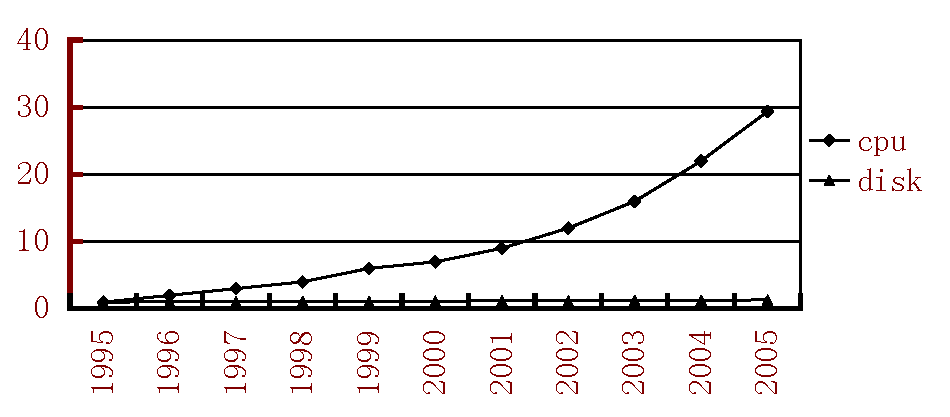
\includegraphics[width=0.7\linewidth]{./graph/cpu-disk-gap}
\caption{CPU与磁盘速度差异}
\label{fig:cpu-disk-diff}
\end{figure}

云端计算\cite{jimgray2003cloud}是计算机系统继从上个世纪八十年代的大规模计算机到“服务器到客户端”计算组织方式的又一次转变。云端计算的对象,大数据(Big Data),因此也获得了存储设备厂商越来越多的关注。大数据之所以出现,是因为我们生活在一个拥有海量数据的信息社会中,21世纪,人们与数据或信息交互比历史上的任何时期都要活跃。46亿全球移动电话用户中,有20亿人访问互联网,人们在畅游互联网的过程中,会自觉或不自觉地产生日志、访问历史和评论等信息,全球互联网每年的数据流量已经达到了713艾字节。除了来自互联网,数据还渗透到了几乎所有行业的所有职能领域,并逐渐晋级为即石油之后又一重要的生产因素。全球知名咨询公司麦肯锡于2011年5月发布了一份题为《大数据:创新、竞争和生产力的下一个新领域》的专题报告,该报告指出:对于大数据的运用预示着人类社会新一波生产效率增长和下一波消费者购买力浪潮的到来。

海量数据的存储和处理对于系统的存储容量、IO速度和运行可靠性提出了非常高的要求,一些高性能的存储设备由此产生。固态硬盘因其诸多优势正逐渐被引入以机械硬盘为主导的传统存储系统中\cite{morris2003evostorage}。从表\ref{tab:ssd-speed-compare}可以看出,固态硬盘的IO性能,尤其是读性能,远高于机械硬盘\cite{libo2010cacheforssd},引入固态硬盘到传统存储系统可在一定程度上提高系统的I/O性能。

\begin{table}[H]
\centering
\caption{HDD、DRAM和SSD的读写速度比较}
\begin{tabular}{|c|c|c|c|}
\hline  & Hard Disk & DRAM & SSD \\
\hline Read Access & 8.3ms & 60ns & 85ns \\
\hline Write Access & 9.1ms & 60ns & 4-10ms \\
\hline
\end{tabular}
\label{tab:ssd-speed-compare}
\end{table}

然而,固态硬盘的价格仍然相对昂贵。固态硬盘的价格在过去2年里一直处于下降的趋势,但这一趋势的脚步正在放慢\cite{henry2014ssdprice},微电子制造工艺和成本问题导致了固态硬盘和机械硬盘之间的价格差距仍会保持很长的一段时间。因此,在短时间内固态硬盘难以取代机械硬盘成为数据中心的首选储存设备。

从2006年和2007年的3美元/GB,固态硬盘的价格已经跌至了目前的0.67美元/GB,但和传统机械硬盘的0.09美元/GB仍存在7倍的差距。通过固态硬盘价格的历史下降速度可以推算出2020年其的价格约为0.14美元/GB,同样计算方法得出的机械硬盘价格将会是0.03美元/GB。此时,对存储厂商来说机械硬盘仍然存在难以抗拒的价格优势。

综上所述,鉴于固态硬盘的价格相对较高这一现状,目前完全使用固态硬盘替代机械硬盘作为存储设备的条件还不够成熟。虽然已有一些云计算存储中心部署了全固态硬盘的存储阵列,但是过高的成本令大多数使用者望而却步。为此,本文设计了一种既能保证成本在可接受的范围内,又能充分利用固态硬盘高I/O性能的缓存系统解决方案。

\section{相关研究工作}
\label{sec:related_works}

针对固态硬盘价格高、功耗低、容量小、读写性能高等特点,很多公司和研究者面向固态硬盘的使用场景,提出了一些基于固态硬盘的混合存储或缓存存储的解决方案。这些方案相比全固态硬盘的解决方案从价格上更能被接受。同时,相比于使用DRAM作为缓存,固态硬盘有着掉电数据不会丢失、运行功耗低(表\ref{tab:ssd-power-compare})\cite{taeho2006flashcache}、存储密度高、接口易于扩展的优势。

\begin{table}[H]
\centering
\caption{DRAM、Flash功耗比较}
\begin{tabular}{|c|c|c|c|}
\hline
\diagbox{介质}{功耗} & Density-Gb/cm2 & Active Power* & Idel Power* \\
\hline DDR2 DRAM & 0.7 & 878mW & 80mW \\
\hline NOR & 0.75 & 86mW & 16μW \\
\hline NAND & 1.42 & 28mW & 6μW \\
\hline
\end{tabular}
\\ * Power consumed for 1Gbit of memory
\label{tab:ssd-power-compare}
\end{table}

全球第六大企业软件公司EMC在2012年推出了VFCache解决方案\cite{vfcache}。该解决方案通过将EMC自处研发的VFCache缓存软件与硬件厂商LSI退出的PCIe闪存适配器系列LSI Nytro WarpDrive卡相结合,从而加速应用性能,改善了该存储环境下刀片服务器的响应时间。VFCache通过拦截不超过64KB大小的读写请求(通常为随机操作)并将其缓存到PCIe闪存卡,达到加速访问的效果。由于不缓存应用程序的写操作,而是直接通过FCHBA卡写入后端SAN存储并等待其反馈成功信息,因此,即使VFCache出现硬件故障也不会导致数据丢失。通过将固态硬盘引进存储阵列,EMC成为第一家涉足服务器PCIe闪存市场的主流厂商。

华为云计算部门的存储技术研发中心提出了SmartCache解决方案\cite{smartcache}。SmartCache是一种将固态硬盘作为缓存资源的分层存储技术,是华为服务器集群所使用的一种动态数据缓存解决方案。SmartCache通过将SSD充当内存扩展的方式,显著降低访问延迟并加快随机IO敏感性应用程序的执行速度,而无需以文件的形式将数据移动到固态硬盘上。SmartCache使用两个或两个以上的固态硬盘作为磁盘阵列的缓存,称为缓存池。在运行中统计机械硬盘上经常访问的热点数据,在系统负荷不高或空闲时,移动磁盘阵列中数据到缓存池中。当访问被移动了的热数据时,SmartCache会直接从缓存池中读取。该方案主要适用于读请求占IO请求的大多数,数据访问位置具有正态分布特性,且长IO请求所占比例不大的场景。

LSI作为一家生产RAID适配器的知名公司,针对混合存储的市场需求,也专门推出了型号为LSI MegaRAID的SATA+SAS RAID控制卡。该控制卡的特点在于集成固态硬盘到RAID卡,使用固态硬盘的空间作为磁盘阵列的缓存,从而有效提高读写性能,降低IO访问时延,降低磁盘阵列重建对性能的影响。结合LSI MegaRAID CacheCade Pro2.0软件\cite{lsiraidcache},无需进行复杂参数配置,就可以将HDD阵列中的热数据动态地拷贝到SSD高速缓存中,操作完全透明。

STEC,一家SAS企业级的闪存驱动器硬件制造商,开源了其自主研发的,Linux系统下的,混合存储软件EnhanceIO\cite{enhanceio},EnhanceIO能够加速任意类型的块存储设备——DAS/RAID/iSCSI/FC SAN。虽然针对STEC自家的产品有优化,EnhanceIO还可支持使用任意品牌和接口型号的固态存储器(包括SAS、SATA、PCIe和Fibre Channel)用作缓存。缓存策略方面,EnhanceIO具备Read Cache(读缓存)、Write Back Cache(写回缓存)和Write-through Cache(写穿缓存)三种模式。EnhanceIO的元数据机制并能够保证用户数据宕机、断电时不会丢失。

另一家SSD生产厂商,STEC的竞争对手Fusion-io也提出了自己的固态硬盘混合存储解决方案Fusion-io ioControl Hybrid Storage Solution\cite{fusionio}。与STEC不同的是,该解决方案针对云计算,能够很好的与虚拟机平台VMware Workstation以及Microsoft SQL Server Clusters整合在一起,提高虚拟机运行速度和减少数据库查询的响应延迟。

\section{全文组织结构}
\label{sec:organization}

为了充分发挥出混合存储系统中高性能硬件对整个系统性能的提升效果,本文提出、实现了一种使用混合存储系统中的固态硬盘作为传统机械硬盘缓存的解决方案。该方案能够在保证数据一致性和对原有系统影响最小的前提下,进一步提升混合存储系统的I/O性能。

论文的全文组织结构如下。

第一章:绪论。论述当前云计算和海量数据处理需求的背景下,对于存储系统提出的新的挑战,以及固态硬盘和机械硬盘这一类型混合存储系统的发展现状。简要描述国内外企业和学术界的相关研究成果、论文的研究意义以及全文组织结构。

第二章:相关技术简介。介绍与论文关系紧密的相关软硬件技术,包括固态硬盘的原理和特性、缓存系统的发展和评估、混合存储系统的原理和分类。

第三章:关键技术。详细介绍实现论文提出解决方案实现过程中所涉及的关键技术,包括磁盘IO的捕获方式、缓存系统使用的页面替换算法、缓存空间的映射策略和缓存块使用的索引结构以及缓存系统提供的两种回写策略。

第四章:缓存系统的具体实现。描述论文抽象出的缓存页面替换算法的公共接口,并对每个接口的具体实现细节加以介绍。介绍磁盘IO捕获函数的内部实现细节。用户配置工具提供的配置参数,以及缓存系统的其他实现细节。

第五章:实验和结果分析。从运行数据一致性和性能提升两个角度对实现的系统进行评估,记录产生的评估结果。与商业缓存软件进行比较,对比缓存系统对机械硬盘的性能提升比例。

第六章:总结与展望。总结论文的研究成果和解决方案的贡献,展望进一步提升系统性能的可行方案。

%% ----------------------------------------------------------------------
%%% END OF FILE
%% ----------------------------------------------------------------------